\header{
    \headtitle{Hymne des faluchards} \label{hymne-des-faluchards}
    %
    
    \insertComment{Sur l'air de "Cadet Rousselle".}{Cadet Rouselle fut écrite en 1792 par Gaspard de Chenu.}
}

\enluminure{4}{\href{https://www.youtube.com/watch?v=KI1CNqp3eE4}{S}}{alut} c'est nous les faluchards
\\De toutes les villes, toutes les régions
\\Salut c'est nous les faluchards
\\De toute la France, nous venons
\\Comptez sur nous pour faire la fête
\\Vous en ferez une drôle de tête
\\Ah, ah les faluchards, sacrés Barbares, sacrés Fêtards !!!
\\\\Salut c'est nous les faluchards
\\Toujours dans l'coup, jamais à part
\\Salut c'est nous, on vient vous voir
\\Vous nous connaîtrez tôt ou tard
\\Et si un soir vous en avez marre
\\Venez nous retrouver dans un bar
\\Ah, ah les faluchards, sacrés Barbares, sacrés Fêtards !!!
\\\\Salut c'est nous les faluchards
\\Les rois d'la bière et du pinard
\\Les princes du Gin et d'la Vodka
\\Rien n'nous fait peur, on aime tous boire
\\Alka Seltzer nous garde vivants
\\Guronsan dans not'verre à dents
\\Ah, ah les faluchards, sacrés Barbares, sacrés Fêtards !!!
\\\\Salut c'est nous les faluchards
\\Bons dans la vie, bons au plumard
\\Et bien des fois il n'est pas rare
\\Qu'on succombe d'un tel panard
\\Jamais en reste, jamais une veste
\\Nous n'avons qu'à faire un geste...
\\Ah, ah les faluchards, sacrés Barbares, sacrés Fêtards !!!
\breakpage
Salut c'est nous les faluchards
\\Etudes, exams on est paré
\\On est tranquille, on est peinard
\\L'essentiel, c'est d'y arriver
\\Insignes, étoiles sont là pour ça
\\Plus on en a plus on aime ça
\\Ah, ah les faluchards, sacrés Barbares, sacrés Fêtards !!!
\\\\Salut c'est nous les faluchards
\\La faluche est notre fierté
\\Et si certains trouvent ça bizarre
\\Ils pourraient goûter de not'pied
\\Partenaire de toutes les fêtes
\\Elle ne quitte jamais notre tête
\\Ah, ah les faluchards, sacrés Barbares, sacrés Fêtards !!!
\\
\bigskip
\begin{center}
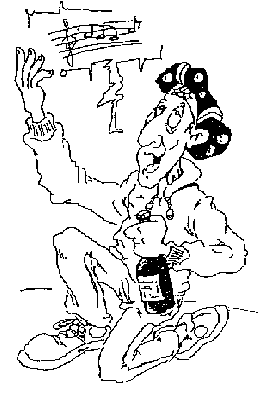
\includegraphics[width=0.6\textwidth]{images/Hymne.PNG}
\end{center}

\breakpage